%%%%%%%%%%%%%%%%%%%%%%%%%%%%%%%%%%%%%%%%%%%%%%%%%%%%%%%%%%%%%%%%%%%%%%%%%%%%%%%%%%
%%																				%%
%% File name: 		10max.tex													%%
%% Project name:	Hochleistungsantenne										%%
%% Type of work:	T3X00 project work											%%
%% Author:			Sarah Brückner, Maximilian Stiefel, Hannes Bohnengel		%%
%% Date:			27th Arpil 2016												%%
%% University:		DHBW Ravensburg Campus Friedrichshafen						%%
%% Comments:		Created in gedit with tab width = 4							%%
%%																				%%
%%%%%%%%%%%%%%%%%%%%%%%%%%%%%%%%%%%%%%%%%%%%%%%%%%%%%%%%%%%%%%%%%%%%%%%%%%%%%%%%%%

\chapter{Hintergründe}

\section{Bahnmechanik}
Es sei zu Beginn diese Absatzes darauf hingewiesen
\subsection{Die Keplerschen Gesetze}
\label{subsec:kepler}
Seit der Antike galt die Erklärung der Bewegung der Planeten und die Vorhersage dieser als eine große Herausforderung. Theorien von Ptolemaios mit seinem geozentrischen Weltbild und Kopernikus mit seinem heliozentrischen Weltbild führten bereits im 16. Jahrhundert zu brauchbaren Modellen zur Vorhersage der Planetenbewegungen. Diese Modelle unterlagen jedoch Ungenauigkeiten, „die in mit Instrumenten des 16. Jahrhunderts bereits messbaren Breichen lagen“ (siehe S. 20 in \cite{Raumflugm}). 
%%%%%%%%%%%%%%%%%%%%%%%%%%%%%%%%%%%%%%%%%%%%%%%%%%%%%%%%%%%%%%%%%%%%%%%%%%%%%%%%%%%%%%%%%%%%%%
\begin{figure}[h]                                                                           %%
	\centering                                                                            	%%
	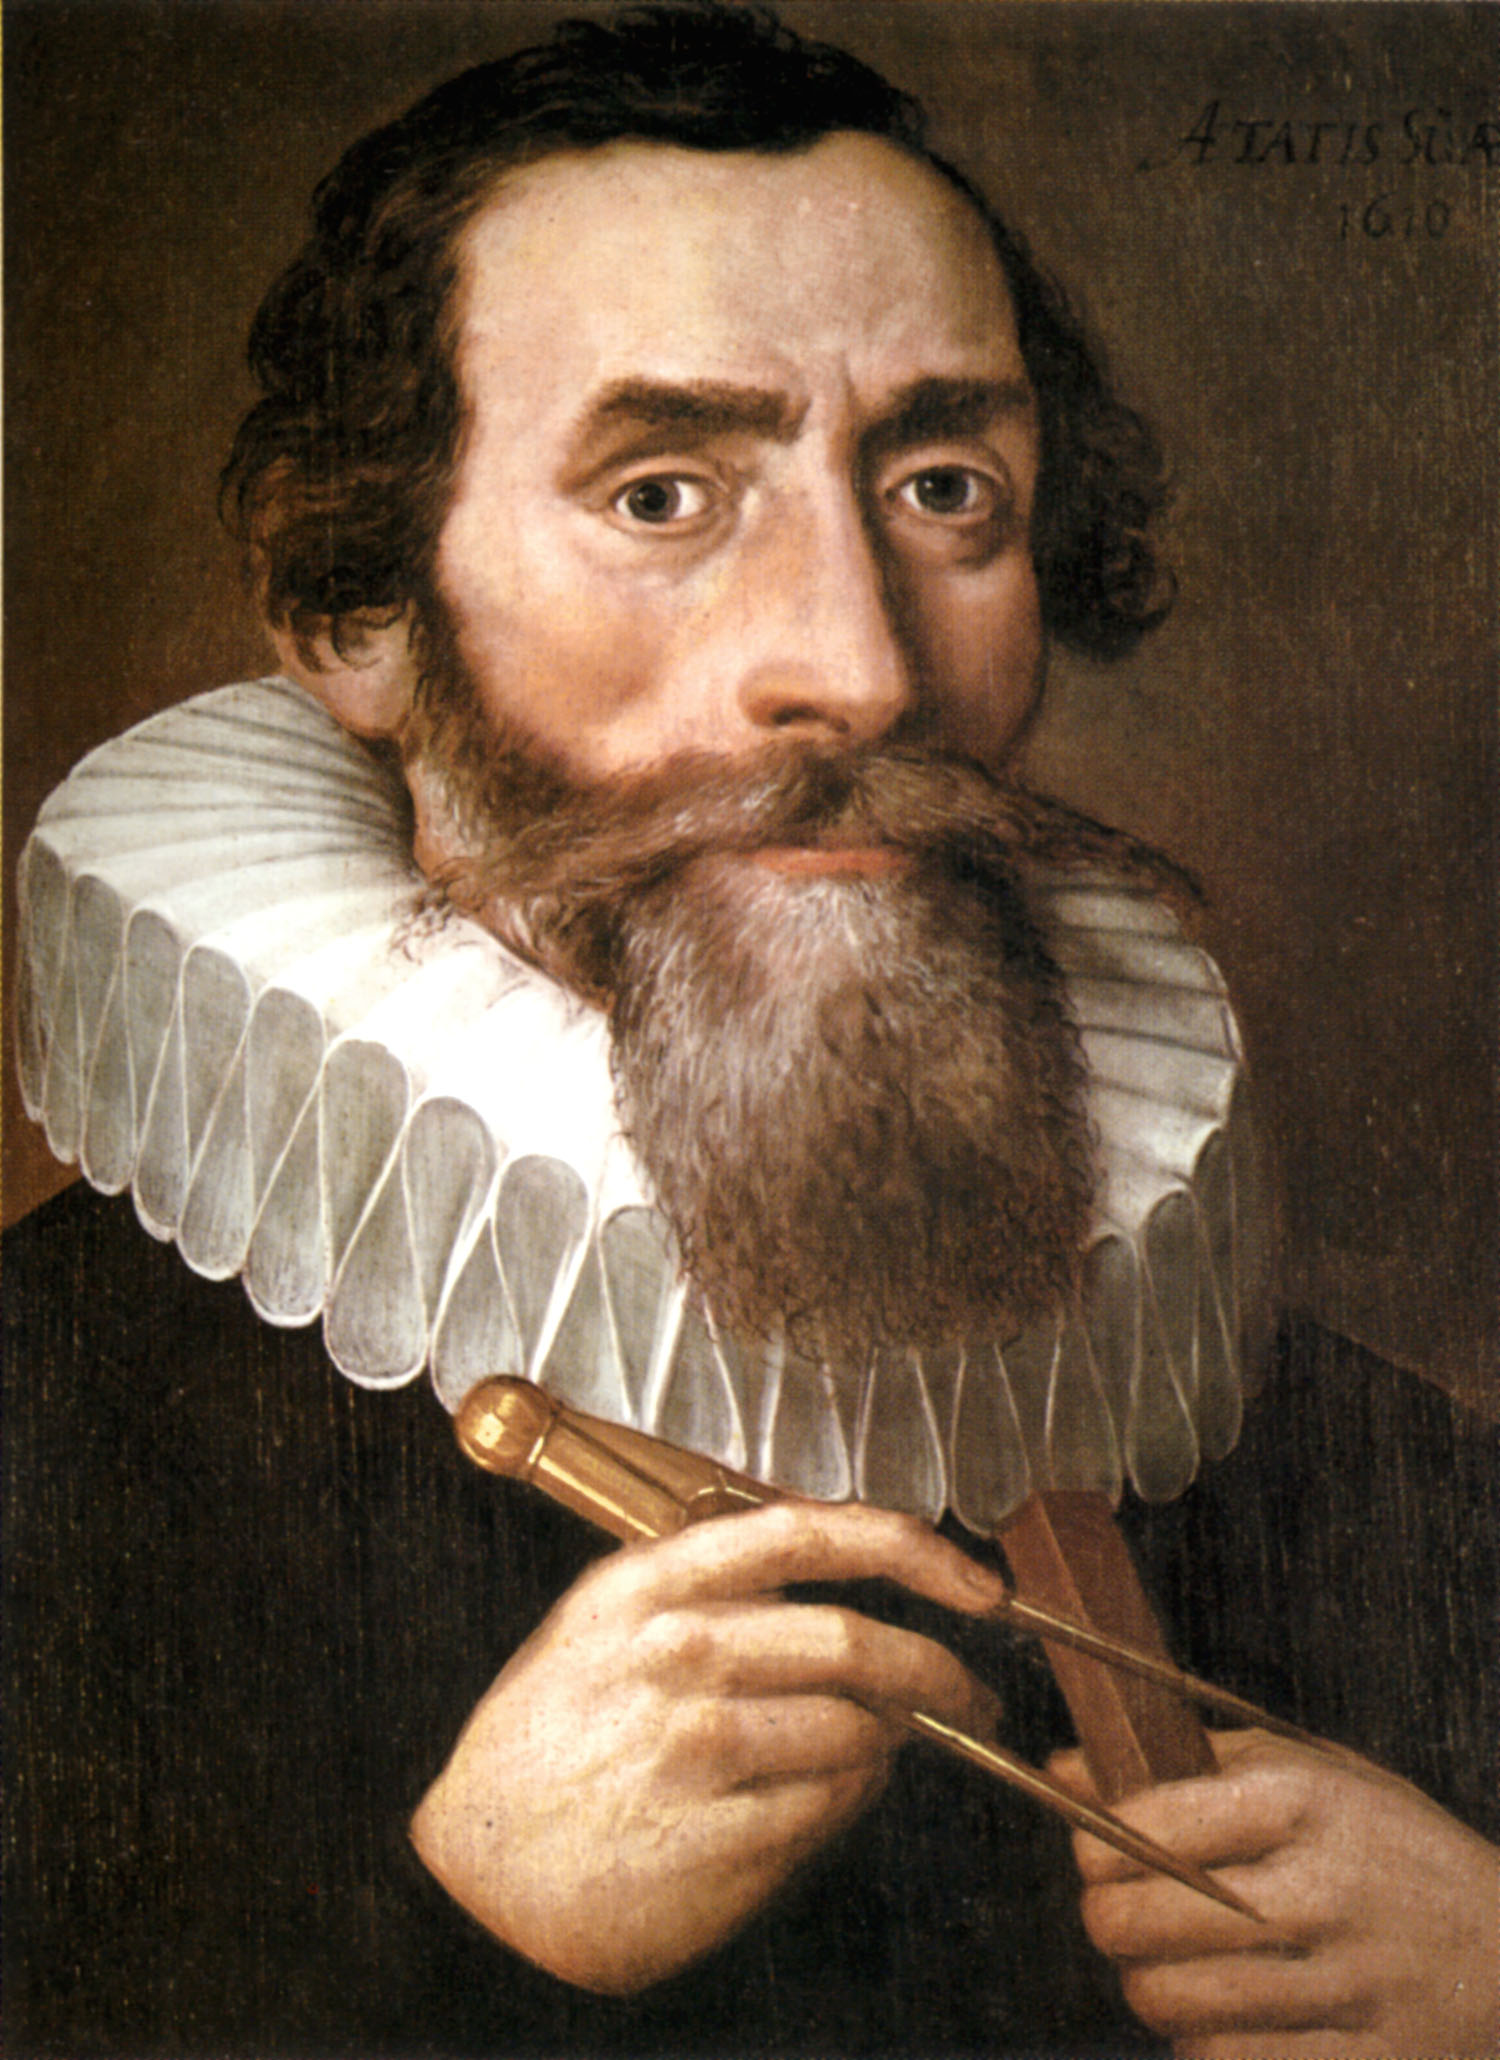
\includegraphics[width=0.3\textwidth]{./images/kepler.jpg}                              %%
	\caption[Bahnelemente]{Johannes Kepler (1571-1630), Quelle: \cite{Wiki:Kepler}}         %%
	\label{fig:bahnelemente}                                                                %%
\end{figure}                                                                              	%%
%%%%%%%%%%%%%%%%%%%%%%%%%%%%%%%%%%%%%%%%%%%%%%%%%%%%%%%%%%%%%%%%%%%%%%%%%%%%%%%%%%%%%%%%%%%%%% 
Der mathematische Aufwand hinter diesen Modellen war enorm. Selbst das kopernikanische Weltbild, dass einige Vereinfachnugen mit sich brachte, bediente sich der Überlagerung einer Vielzahl von Kreisbwegungen, um das Verhalten der Planeten zu erklären. Resignierend zog sich zu der Zeit die katholische Kirsche und mit ihr viele Gelehrte auf den Standpunkt zurück, dass „die Frage, welche der Theorien die korrekte sei, [...] schlicht unbeantwortbar“ wäre (siehe S. 21 in \cite{Raumflugm}). 
\newpar
Ein deutscher Mathematiker und Astronom, Johannes Kepler, war hier anderer Auffassung. Er war überzeugter Kopernikaniker und stand im Dienste des Kaisers Rudolph II. Schließlich gelang es ihm aus seinen Beobachtungen drei einfache Gesetze herzuleiten. Seine Gesetze führten zu Vorhersagen der Planetenbewegungen nie da gewesener Präzision, welche er seinem Dienstherr widmend in den Rudolphinischen Tabellen niederschrieb. Steiner und Schlagerl schreiben in Ihrem Buch „Raumflugmechanik“, dass ohne die Vorarbeit Keplers keine Weltraumtechnik je existiert hätte (vgl. S. 21 in \cite{Raumflugm}). Die drei Gesetze lauten:
\begin{enumerate}
	\item Keplersches Gesetz: Die Planeten umlaufen die Sonne auf elliptischen Bahnen. In einem der Brennpunkte dieser Ellipsen befindet sich die Sonne. 
	\item Keplersches Gesetz: Die Linie von der Sonne zu einem Planeten überstreicht in gleichen Zeiten gleiche Flächen.
	\item Keplersches Gesetz: Die Quadrate der Umlaufzeiten zweier Planeten verhalten sich zueinander so wie die Kuben der großen Halbachsen ihrer Bahnellipsen. 
\end{enumerate}   
Kepler starb 1630 und damit 12 Jahre vor Isaac Newtons (1642-1726) Geburt. Mit seinen Werken hinterließ Kepler Newton alles, um das Gravitationsgesetz später herleiten zu können. 
\subsubsection{Das erste Keplersche Gesetz}
Durch die Annahme Planeten bewegen sich auf Ellipsen anstatt auf Kreisen, brach Kepler ein tausende Jahre altes Paradigma. Das mit der Ellipse war allerdings nicht seine Idee. Bereits im 11. Jahrhundert nahm ein arabischer Gelehrter namens Al-Zarkali (1029-1087) eine elliptische Bahn an, um die unregelmäßige Bewegung des Merkurs erklären zu können. Kepler kannte diese Idee durch die Lehren des Mathematikers und Astronomen Peuerbach (1423-1461), welcher die Ellipsen-Theorie im Abendland verbreitete.  
\newpar
Zunächst soll die Ellipse an sich betrachtet werden. Die einfachste Möglichkeit eine Ellipse zu konstruieren besteht darin zwei Nägel in einer Holzplatte mit einem Stück Schnur mit einer Schlaufe zu verbinden. Das Stück Schnur muss länger sein als der Abstand zwischen beiden Nägeln. Nimmt man nun einen Bleistift und drückt ihn in der Schlaufe gegen die Schnur, kann man die beiden Nägel mit Kontakt der Bleistiftspitze zum Holzbrett umrunden. Hält man die Schnur konstant auf Spannung, so ergibt sich eine Ellipse. Darüber hinaus muss der Punkt auf welchem die Schlaufe am Bleistift anliegt höher sein, als der Abschluss der Nagelköpfe. Im übertragenden Sinne beschreibt die folgende Mengendefinition dieses Experiment mit Bezug zu Abbildung \ref{fig:ellipse}. 
\begin{equation}
E = \{P | \overline{F_{1}P} + \overline{F_{2}P} = 2a = konstant\}
\end{equation}
\ensuremath{F_{1}} und \ensuremath{F_{2}} heißen Brennpunkte der Ellipse. \ensuremath{M} ist der Mittelpunkt der Ellipse. \ensuremath{S_{1}} und \ensuremath{S_{2}} sind die Haupt-, \ensuremath{S_{3}} und \ensuremath{S_{4}} die Nebenscheitel.      
%%%%%%%%%%%%%%%%%%%%%%%%%%%%%%%%%%%%%%%%%%%%%%%%%%%%%%%%%%%%%%%%%%%%%%%%%%%%%%%%%%%%%%%%%%%%%%
\begin{figure}[h]                                                                           %%
	\centering                                                                            	%%
	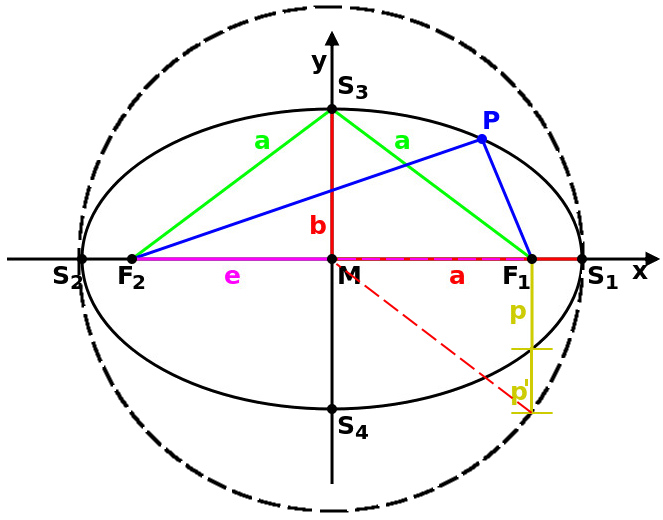
\includegraphics[width=0.6\textwidth]{./images/ellipse_new.jpg}                         %%
	\caption[Ellipse]{Ellipse, Quelle: Wikipedia zusätzlich eigener Überarbeitung}          %%
	\label{fig:ellipse}                                                                     %%
\end{figure}                                                                              	%%
%%%%%%%%%%%%%%%%%%%%%%%%%%%%%%%%%%%%%%%%%%%%%%%%%%%%%%%%%%%%%%%%%%%%%%%%%%%%%%%%%%%%%%%%%%%%%%      
Die Strecke \ensuremath{\overline{MS_{1}}} ist gleich der Strecke \ensuremath{\overline{MS_{2}}}. Man spricht bei der Länge dieser Strecke von der \textbf{großen Halbachse a}. Beide Strecken ergeben zusammen die Hauptachse \ensuremath{\overline{S_{1}S_{2}}}. Analog gibt es hierzu die Nebenachse, welche durch die Strecke \ensuremath{\overline{S_{3}S_{4}}} bestimmt wird. Die \textbf{kleinen Halbachsen} sind \ensuremath{\overline{MS_{3}}} und \ensuremath{\overline{MS_{4}}}. Diese haben die Längen \textbf{b}. Eine Ellipse kann auch als Stauchung eines Kreises mit dem Faktor \ensuremath{\frac{b}{a}} angesehen werden. 
\newpar
Die numerische Exzentrizität e' ist ein Maß für die Schlankheit der Ellipse. Sie ist definiert als
\begin{equation}
	e'=\frac{e}{a}
\end{equation}
Je größer die lineare Exzentrizität e im Verhältnis zu der großen Halbachse a wird, desto schlanker wird die Ellipse, da die Brennpunkte weiter vom Mittelpunkt entfernt sind. Das Wort numerisch gibt bei der Exzentrizität e' an, dass diese sich auf eine andere Größe (die große Halbachse) bezieht. Für eine Ellipse gilt \ensuremath{0 < e' < 1}. Für den Fall \ensuremath{e'=e=0} hat die Ellipse die selbe Erscheinung wie ein Kreis, da die Brennpunkte \ensuremath{F_1} und \ensuremath{F_2} im Mittelpunkt \ensuremath{M} liegen. Für \ensuremath{e'=1} entartet die Ellipse zu einer Geraden, da die kleine Halbachse b zu 0 wird. Um das zu zeigen wird die obige Gleichung noch mal herangezogen.
\begin{equation}
e'^2=\frac{e^2}{a^2}=\frac{a^2-b^2}{a^2}=1-\left(\frac{b}{a}\right)^2 
\end{equation} 
\\Des Weiteren besitzt jede Ellipse einen Halbparameter \ensuremath{p}. Geht man davon aus, dass es einen Abstand \ensuremath{p'} gibt, welcher \ensuremath{p} bis zu einer die Ellipse umschließende Kreislinie verlängert, so gelten folgende Gleichungen
\begin{equation}
	\frac{p}{p'}=\frac{b}{a}
\end{equation}
Mit dem Satz eines alten Freudes folgt
\begin{equation}
p' = \sqrt{a^2-e^2}
\end{equation}
Jetzt ist klar, dass gilt
\begin{equation}
p=\frac{b}{a} \cdot p'= \frac{b}{a} \sqrt{a^2-e^2} = \frac{b^2}{a}
\label{equation_kepler_simple_p}
\end{equation}

Was nun noch fehlt ist „eine Gleichung, also eine analytische Beschreibung der Punkte einer Ellipse“ (siehe S.22 in \cite{Raumflugm}). Eine solche Gleichung ergibt sich mit dem Schnitt einer Ebene mit einem Kegel. 
%%%%%%%%%%%%%%%%%%%%%%%%%%%%%%%%%%%%%%%%%%%%%%%%%%%%%%%%%%%%%%%%%%%%%%%%%%%%%%%%%%%%%%%%%%%%%%
\begin{figure}[h]                                                                           %%
	\centering                                                                            	%%
	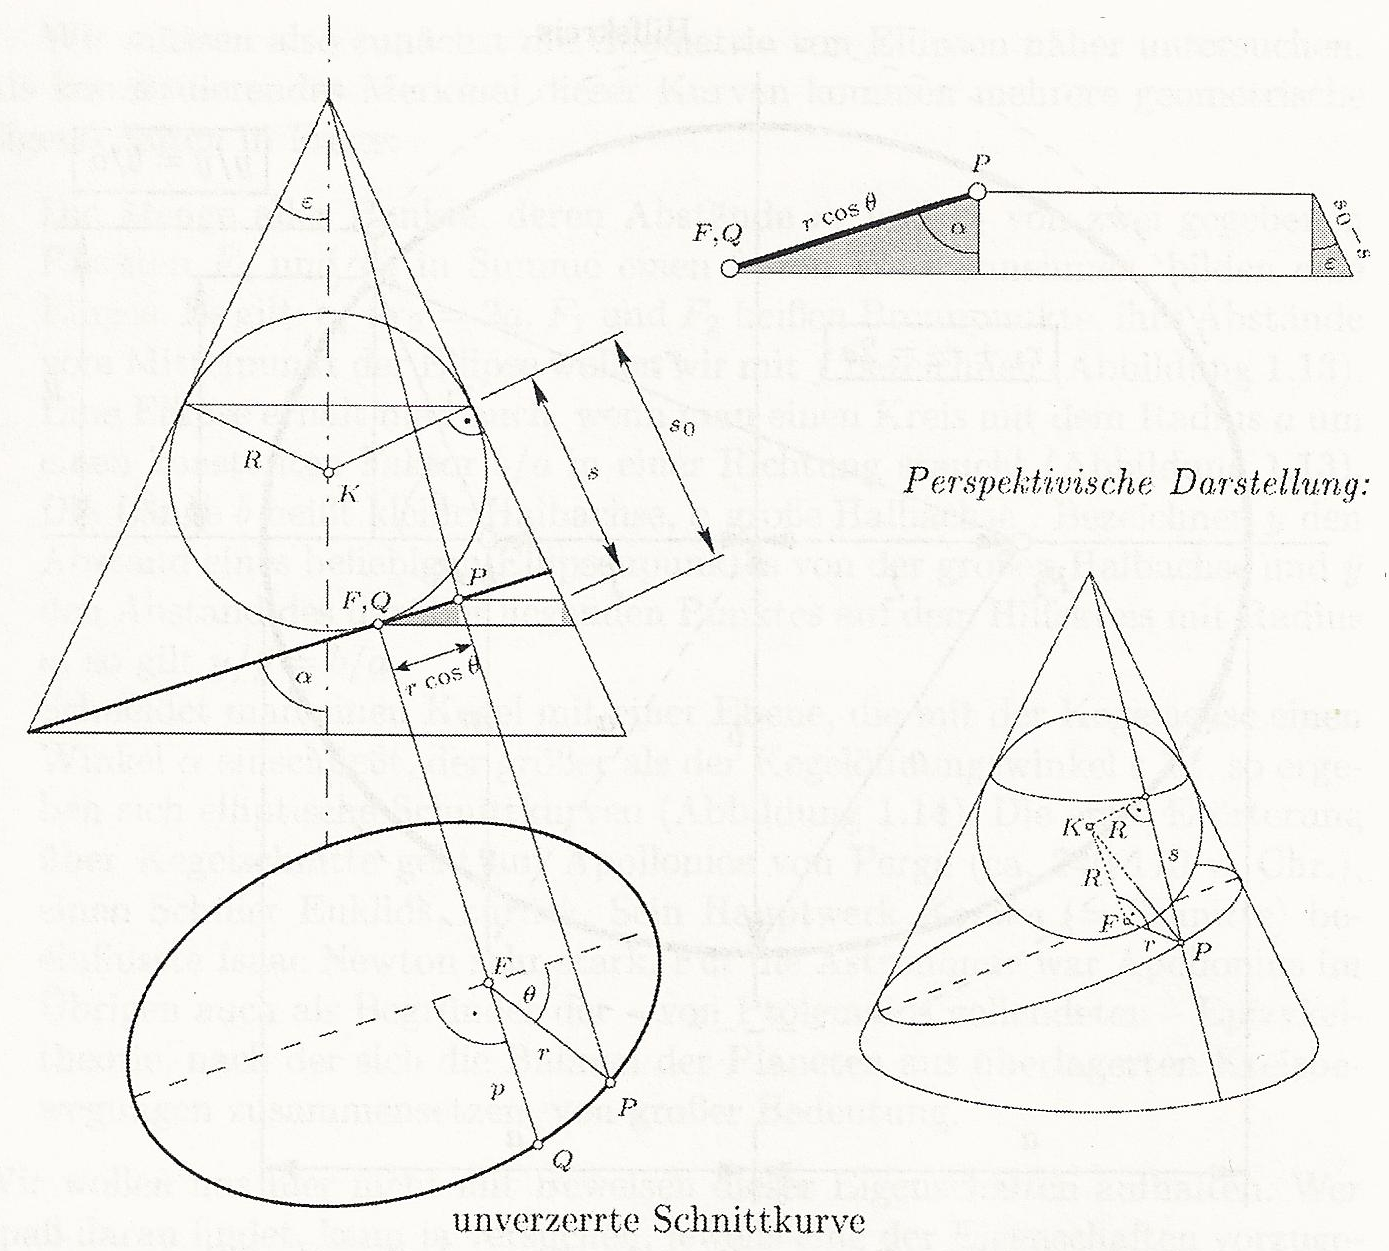
\includegraphics[width=0.8\textwidth]{./images/keplers_law1.jpg}                        %%
	\caption[Kegelschnitt]{Kegelschnitt, Quelle: S.24 in \cite{Raumflugm}}                  %%
	\label{fig:kegelsch}                                                                    %%
\end{figure}                                                                              	%%
%%%%%%%%%%%%%%%%%%%%%%%%%%%%%%%%%%%%%%%%%%%%%%%%%%%%%%%%%%%%%%%%%%%%%%%%%%%%%%%%%%%%%%%%%%%%%%      
Die Neigung der Schnittebene zur Kegelgrundfläche sei \ensuremath{\alpha}. Der Öffnungswinkel des Kegels sei \ensuremath{\epsilon}. Jetzt passiert etwas, dass das räumliche Denkvermögen herausfordert. In den Kegel wird eine (Dandelinsche) Kugel eingeschrieben. Diese Kugel berühre die Ebene im Punkt \ensuremath{F} und tangiere den Kegelmantel entlang eines Breitenkreises. Es ist einzusehen, dass der Punkt \ensuremath{F} auf der Hauptachse der Ellipse liegt. Der Schnittpunkt der entstehenden Ellipse und der Normale zur Hauptachse im Punkt \ensuremath{F} ist der Punkt \ensuremath{Q}. \ensuremath{P} stellt einen beliebigen Punkt auf der Ellipse dar. Die Verbindungslinie zwischen \ensuremath{F} und \ensuremath{P} hat zur Hauptachse die Neigung \ensuremath{\theta}. Der Abstand zwischen \ensuremath{F} und \ensuremath{P} ist \ensuremath{r}. \ensuremath{s} und \ensuremath{s_0} sind die Abstände der Punkte P und Q zum Berührkreis der Kugel gemessen entlang des Kegelmantels. 
\newpar
Man sieht nun, dass die Größen \ensuremath{r}, \ensuremath{s} und \ensuremath{\theta} von P abhängig sind. Es interessiere nun die mathematische Funktion \ensuremath{r(\theta)}, welche die Ellipsenbahn beschreibe (vgl. S.23 in \cite{Raumflugm}). Betrachtet wird nun zunächst die zweidimensionale Zeichnung rechts oben in Abb. \ref{fig:kegelsch}. Mit ein bisschen Nachdenken sieht man, dass
\begin{equation}
	(s_0-s) \cdot cos(\epsilon) = r \cdot cos (\theta) \cdot cos(\alpha)
	\label{equation1_kepler}
\end{equation} 
Doch woher kommt der Ausdruck \ensuremath{r \cdot cos(\theta)}? Hierzu werfe man einen Blick auf die zweidimensionale Abbildung der Schnittfläche/Ellipse links unten im Bild. Dieses Bild setze man nun in Relation zum Bild darüber. Der Abstand \ensuremath{r \cdot cos(\theta)} lässt sich nun auf die Hauptachse der Ellipse projizieren. \ensuremath{r}, die Projektionslinie für P die Hauptachse und F bilden nun eine rechtwinkliges Dreieck aus. Der Rest ist Trigonometrie. 
\newpar
In der Darstellung rechts unten in Abb. \ref{fig:kegelsch} ist folgende Beziehung auffindbar. 
\begin{equation}
 R^2 + s^2 = R^2 + r^2
\end{equation} 
Das bedeutet, dass \ensuremath{s} durch \ensuremath{r} in Gleichung \ref{equation1_kepler} ersetzt werden kann. 
\begin{equation}
	(s_0-r) \cdot cos(\epsilon) = r \cdot cos (\theta) \cdot cos(\alpha)
\end{equation}
Ausmultiplizieren ergibt
\begin{equation}
s_0 cos(\epsilon) - r cos(\epsilon) = r cos (\theta) cos(\alpha)
\end{equation}
Sortieren führt zu 
\begin{equation}
s_0 cos(\epsilon) = r cos (\theta) cos(\alpha) + r cos(\epsilon)
\end{equation}
Ausklammern und auflösen bringt
\begin{equation}
	r = \frac{s_0 cos(\epsilon) }{cos (\theta) cos(\alpha) + cos(\epsilon)}
		\label{equation2_kepler}
\end{equation}
Die entstandene Gleichung \ref{equation2_kepler} kann nun noch durch die Zusammenhänge \ensuremath{p=s_0} (Halbparameter) und \ensuremath{e'=\frac{cos(\alpha)}{cos(\epsilon)}} vereinfacht werden (vgl. S. 24 in \cite{Raumflugm}). Hierzu dividiert man Gleichung \ref{equation2_kepler} durch \ensuremath{cos(\epsilon)}. 
\begin{equation}
r = \frac{s_0}{1+\frac{cos(\alpha)}{cos(\epsilon)}cos (\theta)} = \frac{p}{1 + e' cos(\theta)} 
\label{equation3_kepler}
\end{equation}
Fertig ist die mathematische Version des ersten Keplerschen Gesetzes. 

\subsubsection{Das zweite Keplersche Gesetz}
%%%%%%%%%%%%%%%%%%%%%%%%%%%%%%%%%%%%%%%%%%%%%%%%%%%%%%%%%%%%%%%%%%%%%%%%%%%%%%%%%%%%%%%%%%%%%%
\begin{figure}[h]                                                                           %%
	\centering                                                                            	%%
	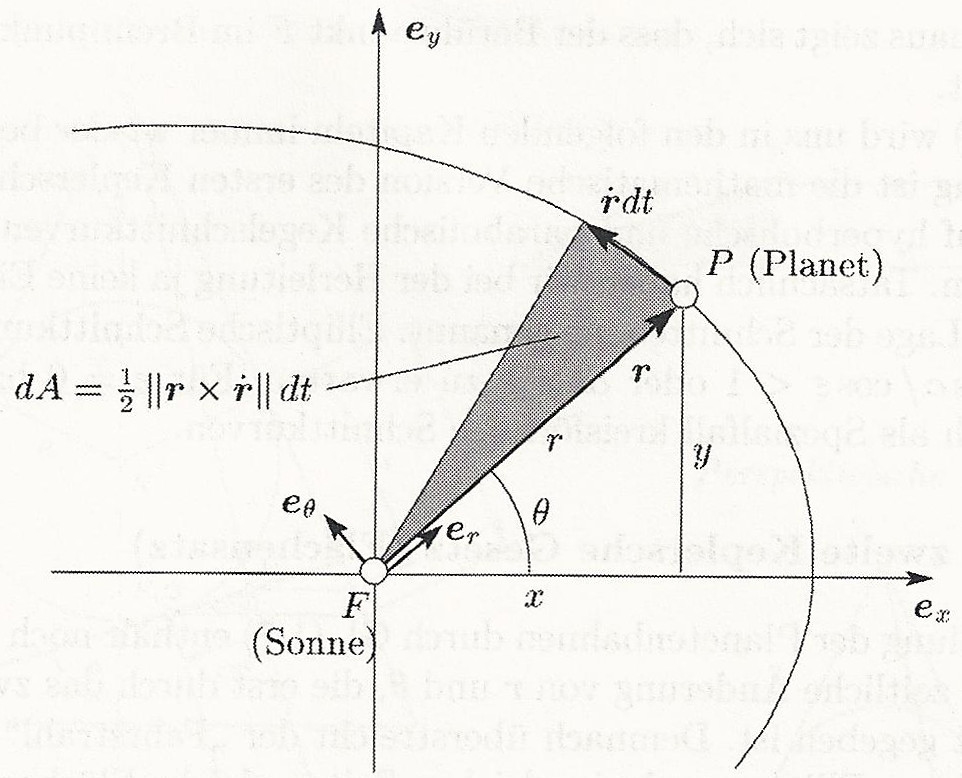
\includegraphics[width=0.6\textwidth]{./images/keplers_law2.jpg}                        %%
	\caption[Kegelschnitt]{Kegelschnitt, Quelle: S.26 in \cite{Raumflugm}}                  %%
	\label{fig:kegelsch}                                                                    %%
\end{figure}                                                                              	%%
%%%%%%%%%%%%%%%%%%%%%%%%%%%%%%%%%%%%%%%%%%%%%%%%%%%%%%%%%%%%%%%%%%%%%%%%%%%%%%%%%%%%%%%%%%%%%%      
Gleichung \ref{equation3_kepler} liefert noch keine Aussage über die zeitliche Änderung von \ensuremath{r} und \ensuremath{\theta}. Um eine Aussage über die zeitliche Änderung dieser Variablen treffen zu können, kann Keplers zweites Gesetz herangezogen werden: Die Fläche, welche die Verbindungslinie zwischen Sonne und einem Planet überstreicht ist zeitlich konstant. Die Fläche \ensuremath{\Delta A}, die in einem Zeitintervall \ensuremath{\Delta t} durch strichen wird ist genau
\begin{equation}
	\Delta A = \frac{1}{2}\left| \vec{r} \times \dot{\vec{r}} \right|\Delta t + F(\Delta t^2)
\end{equation}   
Die beiden Vektoren \ensuremath{r} und \ensuremath{\dot{r} \Delta t} spannen eine Fläche auf, welche ein Parallelogramm beschreibt. Das Kreuzprodukt ergibt einen Vektor dessen Länge dieser Fläche entspricht. Die Hälfte davon ist die Fläche des Dreiecks, die gesucht wird. Der Ausdruck \ensuremath{\dot{r} \Delta t} ist dabei sehr ungenau und beschreibt eigentlich nur die Änderung des Vektors \ensuremath{r}. Aus diesem Grund kommt noch der Fehlerterm \ensuremath{F} hinzu, der die Krümmung der Ellipse berücksichtigt. Bezieht man sich im nächsten Schritt auf infinitesimale Elemente, die wirklich gegen Null gehen, so erreicht man die gewünschte Genauigkeit. Der Fehlerterm wird überflüssig.  
\begin{equation}
dA = \frac{1}{2}\left| \vec{r} \times \dot{\vec{r}} \right|d t 
\label{equation_dA_kepler}
\end{equation}  
Man führt nun eine für jeden Planeten individuelle Konstante \ensuremath{h} ein, da sich das Verhältnis \ensuremath{\frac{dA}{dt}} nicht verändern darf. 
\begin{equation}
2 dA = h \cdot dt 
\end{equation}  
Um das mathematische Äquivalent zu dem sprachlich formulierten zweiten Gesetz zu erhalten, soll wie beim ersten Gesetz eine Abhängigkeit zu \ensuremath{r} und \ensuremath{\theta} hergestellt werden. Zu diesem Zweck wird die Gleichung einer Koordinatentransformation in Zylinderkoordinaten unterworfen (vgl. S. 25 f. in \cite{Raumflugm}). Es gilt also 
\begin{center}
	\ensuremath{x= r\, cos (\theta)}, \ensuremath{y=r\, sin (\theta)} und \ensuremath{z=z}. 
\end{center}
Gemäß der Definition von Zylinderkoordinaten darf man jetzt den Vektor \ensuremath{\vec{r}} auch anders schreiben:
\begin{equation}
	\vec{r} = r\,\vec{e_{r}} + z\,\vec{e_z}
\end{equation}
wobei folgendes generell über Zylinderkoordinatensysteme bekannt ist:
\begin{center}
	\ensuremath{\vec{e_{r}}=\left(\begin{array}{c}cos(\theta)\\ sin(\theta)\\0\end{array}\right)}, \ensuremath{\vec{e_{\theta}}=\left(\begin{array}{c}-sin(\theta)\\ cos(\theta)\\0\end{array}\right)}  und \ensuremath{\vec{e_z}=\left(\begin{array}{c}0\\0\\1\end{array}\right)}
\end{center}
Die Vektoren stehen allesamt senkrecht aufeinander, was man sieht, wenn man das Skalarprodukt bildet. Das liegt daran, dass das Skalarprodukt über die Summe der Längen der Vektoren multipliziert mit dem Kosinus des Winkels den sie einschließen definiert wird, welcher bei \ensuremath{\frac{\pi}{2}} bekanntlich Null ist.Da auch die Ableitung des Vektors \ensuremath{\vec{r}} (Geschwindigkeit) gesucht ist beginnt man zu differenzieren. Man wende hier zunächst die Summenregel, dann auf den ersten Ausdruck noch die Produkt- und die Kettenregel, da \ensuremath{\vec{e_{r}}} von \ensuremath{\theta} abhängt und diese wiederum von \ensuremath{t}. Es folgt
\begin{equation}
	\dot{\vec{r}} = \dot{r}\,\vec{e_r} + r\,\dot{\vec{e_r}} + \dot{z}\,\vec{e_z}
	\label{equation4_kepler}
\end{equation}
Setzt man nun   
\begin{center}	
	\ensuremath{\dot{\vec{e_{r}}}=\dot{\theta}\,\left(\begin{array}{c}-sin(\theta)\\ cos(\theta)\\0\end{array}\right)=\dot{\theta}\,\vec{e_{\theta}}}
\end{center}
in Gleichung \ref{equation4_kepler} ein, so ergibt sich  
\begin{equation}
\dot{\vec{r}} = \dot{r}\,\vec{e_r} + r\,\dot{\theta}\,\vec{e_{\theta}} + \dot{z}\,\vec{e_z}
\label{equation5_kepler}
\end{equation}
Man wählt nun die z-Achse geschickt, so dass diese senkrecht auf der Trägerebene der Ellipse steht (vgl. S.26 in \cite{Raumflugm}). Durch diesen Schachzug gilt für die zu betrachtenden Gleichungen \ensuremath{z=0}. Jetzt fällt Gleichung \ref{equation_dA_kepler} in sich zusammen
\begin{equation}
\frac{dA}{dt} = \frac{1}{2}\left| \vec{r} \times \dot{\vec{r}} \right| = \frac{1}{2}\left| r\,\vec{e_r} \times \left(\dot{r}\,\vec{e_r} + r\,\dot{\theta}\,\vec{e_{\theta}}\right) \right| 
\end{equation}  
Durch die Bilinearität des Kreuzprodukts folgt
\begin{equation}
\frac{dA}{dt} = \frac{1}{2}\left| \dot{r}\,r\,\left(\vec{e_r} \times \vec{e_r}\right) + r\,r\,\dot{\theta}\,\left(\vec{e_r} \times \vec{e_{\theta}}\right) \right| 
\end{equation}
Die Tatsache, dass das Kreuzprodukt eines Vektors mit sich selbst den Nullvektor ergibt und dem Umstand, dass \ensuremath{\vec{e_r}\perp\vec{e_\theta}\perp\vec{e_z}} ist, führt zu
\begin{equation}
\frac{dA}{dt} = \frac{1}{2}\left|r^2\,\dot{\theta}\,\vec{e_z} \right| =  \frac{1}{2}\,r^2\,\dot{\theta}=h=konstant
\label{equation6_kepler}
\end{equation}

\subsubsection{Das dritte Keplersche Gesetz}
Auf sein drittes Gesetz soll Kepler besonders stolz gewesen sein (vgl. S.27 in \cite{Raumflugm}). Nach seinem Gesetz stehen die Halbachsen \ensuremath{a_1} und \ensuremath{a_2} und die Umlaufzeiten \ensuremath{T_1} und \ensuremath{T_2} in dem Zusammenhang
\begin{equation}
	\frac{T_1^2}{T_2^2}=\frac{a_1^3}{a_2^3}
	\label{equation7_kepler}
\end{equation} 
Die Umlaufzeit lässt sich nun leicht mit der Konstanten \ensuremath{h}, welche für das zweite Keplersche Gesetz eingeführt wurde ausdrücken. Es wird hierfür die gesamte Ellipsenfläche (\ensuremath{A_{Ellipse}=ab\pi}) und konsequenterweise dann auch die gesamte Umlaufzeit \ensuremath{T} angenommen. Eingesetzt in Gleichung \ref{equation6_kepler} ergibt sich
\begin{equation}
	2ab\pi=hT.
\end{equation} 
Daraus folgt
\begin{equation}
	T=\frac{2ab\pi}{h}.
\end{equation}
Eingesetzt in Gleichung \ref{equation7_kepler} ergibt sich 
\begin{equation}
		\frac{T_1^2}{T_2^2}=\frac{a_1^3}{a_2^3}=\frac{a_1^2b_1^2h_2^2}{a_2^2b_2^2h_1^2}
\end{equation}
Bringt man nun \ensuremath{a_1^2b_1} und \ensuremath{a_2^2b_2^2} einmal durch Division und einmal durch Multiplikation eins weiter nach links, so kann man die Beziehung aus Gleichung \ref{equation_kepler_simple_p} ausnutzen und schreiben
\begin{equation}
\frac{a_1b_2^2}{a_2b_1^2}=\frac{h_2^2}{h_1^2}
\end{equation}
Oben und unten multipliziert man jetzt noch jeweils mit \ensuremath{1/a_1} und \ensuremath{1/a_2}.
\begin{equation}
\frac{b_2^2/a_2}{b_1^2/a_1}=\frac{h_2^2}{h_1^2}=\frac{p_2}{p_1}
\end{equation}
Das Resultat ist ein „Zusammenhang zwischen den Halbparametern \ensuremath{p_1}, \ensuremath{p_2} und den Bewegungskonstatnten \ensuremath{h_1}, \ensuremath{h_2}“ (siehe S.27 in \cite{Raumflugm}). Diese Größen sind aus dem zweiten Keplerschen Gesetz bekannt. 

\subsection{Die Bahnelemente}
%%%%%%%%%%%%%%%%%%%%%%%%%%%%%%%%%%%%%%%%%%%%%%%%%%%%%%%%%%%%%%%%%%%%%%%%%%%%%%%%%%%%%%%%%%%%%%
\begin{figure}[!htbp]                                                                       %%
	\centering                                                                            	%%
	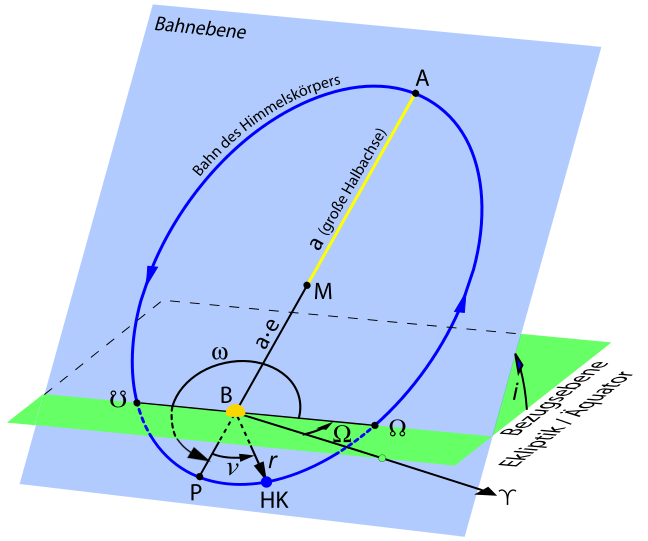
\includegraphics[width=0.8\textwidth]{./images/bahnelemente.png}                        %%
	\caption[Bahnelemente]{Bahnelemente, Quelle: \cite{Wiki:Bahnel}}                        %%
	\label{fig:bahnelemente}                                                                %%
\end{figure}                                                                              	%%
%%%%%%%%%%%%%%%%%%%%%%%%%%%%%%%%%%%%%%%%%%%%%%%%%%%%%%%%%%%%%%%%%%%%%%%%%%%%%%%%%%%%%%%%%%%%%%   
Die Bahnelemente dienen der Beschreibung einer Bewegung eines Himmelskörpers auf einer Umlaufbahn (meist einer Ellipse). Dieser Körper unterliegt den Keplerschen Gesetzen. Wird die Bewegung eines Himmelskörpers durch äußere Einflüsse (z.B. Gravitationskraft der Sonne) nicht gestört, so kann sie durch sechs Größen beschrieben werden. Diese Größen sind die Bahnelemente. Zwei Bahnelemente beschreiben die \textbf{Form der Bahn}, drei legen die \textbf{Lage der Bahn} im dreidimensionalen Raum fest und ein Bahnelement gibt an zu welcher \textbf{Zeit} sich der Himmelskörper wo auf der Bahn befunden hat. 
\newpar
Diese Bahnelemente reichen in der Praxis nicht aus, um die Position eines Himmelskörpers z.B. eines Satelliten mit einem Vorhersagemodell berechnen zu können. Aus diesem Grund werden die Bahnelemente meist um von Vorhersagemodellen benötigten Informationen ergänzt.       
Im Folgenden werden die Bahnelemente in Ihrer Bedeutung anhand der Abbildung \ref{fig:bahnelemente} erläutert. 

\subsubsection{Gestalt der Bahn}
Um die Gestalt der Bahn zu beschreiben wird die \textbf{numerische Exzentrizität \ensuremath{e'}} und die Angabe der Länge der \textbf{großen Halbachse \ensuremath{a}} benötigt. Diese beiden Größen werden ausführlich im Absatz \ref{subsec:kepler} beschrieben. Es braucht nicht mehr, um eine elliptische Bahn zu definieren. Zur Erinnerung: Die große Halbachse \ensuremath{a} ist die Länge der Strecke vom Mittelpunkt zu den Hauptscheiteln. Die (lineare) Exzentrizität \ensuremath{e} gibt die Schlankeit der Ellipse an. Wobei die numerische Exzentrizität \ensuremath{e'} auf die große Halbachse normiert ist.  

\subsubsection{Lage der Bahn}
Es erscheint sinnvoll, dass die Lage im Raum als nächstes festgelegt wird. Auch scheint es sinnig, dass man drei Bahnellemente benötigt, um die Lage der Bahn im dreidimensionalen Raum festzulegen. 
\newpar
Man stelle sich nun vor, dass die Ellipse, auf welcher der Satellit sich bewegt, in einer Ebene liege.  Diese Ebene schneide man mit einer Referenzebene (z.B. Schnittebene durch den Erdäquator). Die \textbf{Inklination \ensuremath{i}} ist nun ein Winkel, „um den die Bahnebene gegenüber der [Referenzebene] geneigt ist“ (siehe S.88 in \cite{HandRaum}). Um die Nebenachse der Ellipse herum kann durch diese Festlegung keine Rotation mehr stattfinden. Die Ellipse, die ja in der Ebene liegt, kann sich jetzt noch in dieser Ebene um eine zur Ebene orthogonalen Achse drehen. Um das zu unterbinden wird ein weiterer Winkel, das \textbf{Argument des Perigäums \ensuremath{\omega}}, eingeführt. Das Argument des Perigäums ist der Winkel, den die Knotenlinie und die Perigäumsrichtung (Hauptachse) einschließen. Das Perigäum liegt am Ende der Hauptachse, auf welches sich der Satellit zu bewegt, nachdem er den aufsteigenden Knoten passiert hat. Der aufsteigende Knoten ist der Punkt in dem der Satellit die Referenzebene auf seiner elliptischen Umlaufbahn (von Süd nach Nord) durchstößt. Die Knotenlinie ist die Schnittgerade der Ellipse mit der Referenzebene. Darüber hinaus gibt es das Apogäum, welches nach dem absteigenden Knoten durchlaufen wird, der am anderen Ende der Nebenachse beheimatet ist. Eine andere Definition für das Perigäum ist der Punkt des geringsten Abstands des Satelliten zur Erde. Analog lässt sich das Apogäum als Punkt des größten Abstands des Satelliten zur Erde festlegen. Die Ellipse dreht sich nun nicht mehr in der Ebene. Eine Sache wurde jetzt noch nicht betrachtet. Die Ebene kann sich immer noch entlang Ihrer Hauptachse drehen. Die \textbf{Rektaszension des aufsteigenden Knotens \ensuremath{\Omega}} gibt nun den Winkel an, den die Knotenlinie und der Vektor vom Ellipsenmittelpunkt zum Frühlingspunkt \ensuremath{\gamma} einschließen. Doch was ist der Frühlingspunkt? „Als Frühlingspunkt (auch Widderpunkt) wird in der Astronomie der Schnittpunkt des Himmelsäquators mit der Ekliptik bezeichnet, an dem die Sonne zum Frühlingsanfang der Nordhalbkugel (= Herbstanfang der Südhalbkugel) steht“ (siehe \cite{Wiki:Frue}). Die Derehung um die Hauptachse ist jetzt also auch nicht mehr möglich. Der Bahnlage wurden somit alle drei Freiheitsgrade genommen.     

\subsubsection{Zeitlicher Bezug}


\section{Vorhersagemodelle}

\clearpage